\documentclass[titlepage]{article}
\usepackage{graphicx}
\usepackage{caption}
\usepackage{textcomp}
\usepackage{subcaption}
\usepackage[margin=0.5in]{geometry}
\usepackage{titling}
\usepackage{csvsimple}
\usepackage{longtable}
\usepackage{booktabs}
\usepackage{float}
\usepackage{cite}
\usepackage{lineno}
\usepackage{natbib,letltxmacro}
\LetLtxMacro\cite\citep 
\linenumbers
\newcommand{\subtitle}[1]{%
  \posttitle{%
    \par\end{center}
    \begin{center}\large#1\end{center}
    \vskip0.5em}%
}


\title{How well do different linear and nonlinear growth models fit to bacterial growth curves?}
\author{Sarah Dobson ,Imperial College London sld21@ic.ac.uk, Word Count: 2600}
\date{27th November 2021}


\begin{document}
  \maketitle
  \section{Abstract}
  
Microbial growth is a common cause of food spoilage and posioning. Mathmatical models that predict the rate of bacterial growth can be used to determine the shelf life of food products, minimise bacterial growth and optimise food production. Both linear and non-linear models have been used to predict growth curves across the literature, however which model is best at fitting bacteria growth curves is still debated. Using datasets from multiple published papers I compared two polynomial linear models: cubic and quadratic, with the three most popular non linear models, the Logistic, Gompertz and the Biryani Models, using AICc values to determine (1) whether linear or non linear models best predict bacterial growth curves and (2) which model best predicts bacterial growth overall. I found that the Gompertz model best fitted bacterial growth curves across the datasets but I could not determine whether linear or non linear models were superior at fitting bacterial growth curves due to convergence issues in the non linear models. Future studies should sample the starting parameters of non linear models in order to get a higher convergence rate.
  
  \section{Introduction}
  
Microbial growth is a common cause of food spoilage and posioning \cite{peleg2011microbial}. Food spoilage may be visible as the growth of slime colonies, textural changes, or off-odors and off-flavors (NRC 1985). Mathmatical models that correctly predict the rate of bacterial growth can be used to predict the shelf life of food products, minimise bacterial growth and optimise food production \cite{baranyi1994dynamic}. Bacterial growth can be separated into 4 phases as shown in Figure 1:
  

 \begin{figure}[H] 
  \centering
  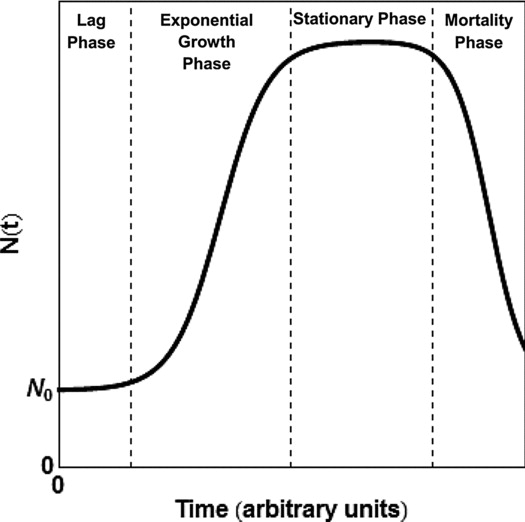
\includegraphics[scale=0.5] {../report/growthcurve.jpeg}
   \label{Figure 1}
    \caption{\footnotesize This diagram,taken from \cite{peleg2011microbial}, shows the four phases of bacterial growth \(N_{t}\) over time: known all togather as the bacterial growth curve. (1) the lag phase: when bacteria are introduced to a new environmrnt or medium they do not initially grow and instead activate genes involved in better nutrient uptake from the new enviroment. (2)the exponential growth phase: acclimitisation to the new environemnt has been completed, and the bacteria starts to grow exponentially. (3)stationary phase: growth wavers as resources start to become limited, eg. competition for food and/or space. (4) death or mortality phase: as resources start to decline, the bacteria start to die off.} 
\end{figure}

Over the years, a number of different models were used to attempt to predict bacterial growth. Two major types of model are used: linear and non linear. Linear models describe the direct relationship between growth and any explanaotry variables(in this case time) by using linear predictor functions whereas non linear models are fit to growth curves based on a minimum number of biologically relevent parameters \cite{grijspeerdt1999estimating}. \\

Traditionally, microbial growth rates were measured by plotting population size against the time since innoculation and fitting a linear regression through the exponential growth phase \cite{whiting1992quantitative, baranyi1994dynamic}. However, this method only looks at predicting bacterial growth in the exponential growth phase and  does not take into consideration the other phases which are also biologically relevant. For example, the duration of the lag phase determines how long food will last before becoming spoiled and in single cells determines when pathogenic cells can multiply to a poisoning concentration level  \cite{baranyi1994dynamic,baranyi2009parameter,olofsson2011modeling}. \\

However, linear polynomial models, using a cubic or quadratic equation, could potentially capture the delayed start of population growth in the lag phase, decreasing momentum of the stationary phase and decline of the death phase. They are also commonly used to assess growth curves in other research fields such as plant growth \cite{jane2019comparison}. Linear models are also easy to run, interperate and \cite{grimm2011nonlinear}. It is possible that bacterial growth is better captured by nonlinear models. Growth rates do not change linearly or reach a maximum  point like polynomial  models \cite{jane2019comparison}. However, they are not as robust as linear models \cite{buchanan1997simple}. \\

Over the years, many studies have used different models to fit bacterial growth curves, with differing conclusions. Therefore, there is significant disagreement in literature on which model is the best for predicting bacterial growth curves and selecting a model to use often appears to be subjective \cite{pla2015comparison}. 
Determining which of the models predicts bacterial growth best can be determined by model selection, where competing models are directly compared to each other and ranked by determining the relative support in the observed data for each model \cite{johnson2004model}. \\

Therefore I will compare two polynomial linear models: cubic and quadratic, with three of the most popular non linear models for predicting bacterial growth \cite{pla2015comparison}: the logistic model, the Gompertz Model and the Baranyi Model. I will fit all of these models across multiple datasets of bacterial growth over time. Using model selection, I will determine (1) whether linear or non linear models best predict bacterial growth curves and (2) out of all the models used which one best predicts bacterial growth.



  \section{Methods}
  
 \subsection {Computing Tools}
All of the data wrangling, model fitting and plotting was completed in R version 3.6.3. I wrangled the data and fitted the models using the tidyverse package \citep{wickham2017tidyverse}, which provided an easy and innutive way to filter and manipulate data and apply model fittins across each dataset. I fitted the linear models using the lm functionin in base R. I fitted the nonlinear models using NLLS (Non linear least squares) using the package minpack.lm \cite{elzhov2016package} which uses non linear least squares to fit data to models with a slight modification to the LevenbergMarquardt algorithm, which creates a more robustness structure that handles less optimal starting parameter values. I calculated the AICc values using the package MuMIn \cite{barton2015package} which easily streamlines the information-theoretic model selection and carries model averaging based on information criteria. I pulled model ouputs into dataframes using the package broom \cite{robinson2014broom}, which made report resulting, creating plots and working with large numbers of models easy. I used a bash script to wrangle the data, fit models, plot the ouputs and compile the results into this pdf file. Bash allows me to easily sequentially run each script with minial coding.


  
  \subsection {Data Manipulation}

I used Datasets from 10 peer-reviewed research papers to test model fits. These datatsets included populations of different bacterial species recorded over time in varying environmental conditions. Therefore, seperate datasets used to test model fits were defined by the paper the dataset came from, the species of bacteria used, temperature the bacteria were grown at, medium the bacteria were grown and the replicate number if the experiment was replicated. This gave a total of 305 datasets. The sample size of each dataset ranged from 3 to 151. I removed datasets with less than 8 datapoints as the models may have trouble fitting small sample sizes. I also removed negative population size and time measurements from datasets because these measurements are biologically impossible and were likely the result of a recording error. 


  \subsection{Model fitting}
  
 \subtitle{Linear models}

  For each dataset I fitted a quadratic regression linear model and a cubic regression linear model in R version 3.6.3. The log population size was the response with the time since innoculation as the explanatory variable. For the quadratic and cubic models time was fitted as a quadratic and cubic affects respectively. All models were checked for goodness of fit and that the assumptions for linear models were met.
  
  
\subtitle{non Linear models}

  
All linear models were fit using a non linear least squares method (NLLS) using the package min.pack.lm \cite{elzhov2016package} in R version 3.6.3. NLLS fits models to data by minimizing the squared differences between observed and predicted values \cite{johnson2004model}. Each model was run with 1000 iterations, the starting values used for each model are specified below. All model were checked for goodness of fit and that the assumptions for non linear models were met. \\

  
  
For my first nonlinear model I fitted each dataset to a logisitc model \cite{verhulst1838notice} with the following equation:

  \begin{equation}
    N_{t} =\frac{N_{0}K_{e}^{rt}}{K + N0(e^{rt}-1)} 
  \end{equation}
  
\(N_{t}\) is the population size at time \(t\), \(t\) is the time since innoculation, \(N_{0}\) is the initial size of the bacteria population, \(K\) is the carrying capacity (ie. the maximum population size that the bacteria can achieve) and \(r\) is the maximum growth rate (the fastest that the bacteria population grows in a given time frame). I used  K, \(N_{0}\) and \(r\) as starting parameters. For each dataset, \(K\) was calculated by determining the maximum population size reached, \(N_{0}\) was calculated by determining the population size at the first datapoint and r was determined by calculating the slope of the log of the population size against time via linear regression. \\



The second model is a revised Gompertz model \cite{grijspeerdt1999estimating}. The gompertz model was fitted to each dataset using the following equation: 
  
  
    \begin{equation}
  log(N_{t}) = log(N_{0}) + (log(K) - log(N_{0})e^{-e*(r*e(1)*\frac{t_{lag} - t}{log(K) - log(N_{0})*log{10}}} +1
   \end{equation}
  
  
The defintions for \(N_{t}\), \(t\), \(N_{0}\),\(K\) and \(r\) are the same as the logisitic model above. \(t_{lag}\) is the amount of time the population spends in the lag phase. In the gompertz model \(r\) is the tangent to the infection point while \(t_{lag}\) intercepts this tangent on the x-axis. For each dataset, \(K\) was calculated by determining the maximum log population size reached, log\(N_{0}\) was calculated by determining the log population size at the first datapoint, \(r\) was determined by calculating the slope of the log of the population size against time via linear regression and \(t_{lag}\) was calculated using the furtherest time point away from the intial time point where there was no growth in population size. \(r\) was calculated using the same methods described for the logistic model. \\


The third linear model is the Baranyi Model \cite{baranyi1994dynamic} which is based on the concept that the  rate of  bacterial growth is controlled  by the rate of a ‘bottleneck’ biochemical reaction \cite{buchanan1997simple}. I fitted the data in each dataset to the Baranyi model using the two equations below taken from \cite{pla2015comparison}. I inserted the equation for \(N_{t}\) into places were \(N_{t}\) appeared in the equation for log\(N_{t}\). 
  
    \begin{equation}
    Equation 1:  log(N_{t}) = N_{0}+r*A*N_{t}*t -ln(1 + \frac{e^{r*N_{0}*t}-1}{e^{(K - N_{0})}}
    \end{equation}
    
    \begin{equation}
    Equation 2: N_{t} = t - \frac{1}{r}*ln*(e^{-r*t}+e^{-r*t_{lag}}- e^{-r(t+t_{lag})})
    \end{equation}
  
  
  
  
The defintions for \(N_{t}\), \(t\), \(N_{0}\),\(K\), \(r\) (and \(t_{lag}\) are the same as the gompertz model.  
  
  
\subsection{Comparing Models}
  
I compared how well each model across fitted the data across each dataset by calculating their small sample unbiased Akaike information criterion (AICc) values  using the package MuMIN \cite{barton2015package} in R. AICc values are ideal for comparing between models as they consider both fit and complexity of the models, and correct biases for more complex models \cite{johnson2004model}. AICc also corrects bias for small sample sizes, and should be used when the total number of samples divided by the number of parameters is less than 40 \cite{johnson2004model}. This is the case for the majority of the datasets. The best fiting model for each dataset was assigned with the model with the lowest AICc. The best fitting model across all the datasets was determined by considering how many times each model successfully converged and the number of times each model had the lowest AICc across all datasets and the total number datasets where they successfully ran. 
  
  
  
\section{Results}
  
In total I fitted each model to 228 datasets. Ranigng from 8 to 151 data points, with 23823 data points across all datasets. Model diagnostics showed that the datasets fit the assumptions for NLLS analysis. A list of all the model AICc and the best fitting model for each dataset can be found in table S1. A list of how many times each model had the lowest AICc and successfully converged across all the datasets are found in Table 1. 

\begin{table}[t]
 \label{Table 1}
\caption{\footnotesize A list of the number times each model was the best fit and successfully converged across all 228 datasets}
\begin{tabular}{lll}
Model     & Best Model Count & Convergence Count \\
Quadratic & 58               & 228               \\
Cubic     & 53               & 228               \\
Logisitc  & 37              & 221               \\
Gompertz  & 75              & 128               \\
Baranyi   & 5               & 26                
\end{tabular}
\end{table}


The quadratic and cubic linear models converged across the most datasets at 100\%, while the logistic, gompertz and baranyi models converged in 97\%, 56\% and 11\% of the datasets respectively (Table 1). Only 4 of the 228 datasets had successful runs with all models. The quadratic and cubic linear models had the best model fit for 25.4\% and 23.3\% of the datasets respectively. The logisitc model was the best fit for 16.7\% of the datasets were the model converged, and 16.2\% overall. The baranyi model was the best fit for 19.2\% of the datasets where the model converged and 2.2\% overall. The gompertz model had the highest number of best fits both across the datasets where the model converged at 58.5\% and across all datasets at 32.9\%.  In total, linear models and non linear models were the best fit for 48.6\% and 51.4\% of the datasets respectviely. ON average the linear and nonlinear models had a best model fit of 55.5\% and 39\% respectively. Plotting model outputs for each dataset visualised how well the models fit the data. Examples of the plotted predicted lines for each dataset are shown in figure 2.

 \begin{figure}[H] 
  \centering
   \label{Figure 2}
\begin{subfigure}{.4\textwidth}
  \centering
  \includegraphics[width=\linewidth]{../results/245_1.pdf}
    \caption{\footnotesize Plots the change in log population size over time for dataset 245\_1 where every model successfully converged. Each line represents a different model. Each datapoint represents individual samples from the dataset.}
  \label{fig2:Figure 2a}
\end{subfigure}
 \hspace{1em}
\begin{subfigure}{.4\textwidth}
  \centering
  \includegraphics[width=\linewidth]{../results/126_1.pdf}
    \caption{\footnotesize Plots the change in log population size over time for dataset '196\_1', where every model except baranyi successfully converged. Eaah line represents a different model. Each datapoint represents individual samples fromm the dataset.}
  \label{fig2:Figure 2b}
\end{subfigure}
\vspace{1em}
\begin{subfigure}{.4\textwidth}
  \centering
  \includegraphics[width=\linewidth]{../results/230_1.pdf}
    \caption{\footnotesize Plots the change in log population size over time for dataset 230\_1,, where only the quadratic, cubic and logisitc models uccessfully converged. Each line represents a different model. Each datapoint represents individual samples from the dataset.}
  \label{fig2:Figure 2c}
\end{subfigure}
\caption{\footnotesize shows plots of the predicted lines for each model across selected datasets}
\label{Figure 2}
\end{figure}


  
\section{Discussion}


I found that while non linear models were the best fitting models fits across more datasets than linear models, on average the linear models accounted for more best model fits than the non linear models. Further examination also reveals that across some datasets, the AICc values of the Gompertz, Quadratic and Cubic models had a difference of less than 2 in (Table S1). An AICc difference of less than 2 is not significantly different and AICcs wihtin that range should all be considered the best fit \cite{akaike1998bayesian}.  \\

None of the non-linear model managed to converge across all datasets. A lack of model convergence suggests that the models are not a good fit to the data. However, the model parameters are based on theoretical phases in closed habitats, which rely on the datasets recording population growth from start to end \cite{grijspeerdt1999estimating}, and that there is sufficient information recorded for each phase \cite{buchanan1997simple}. The death phase is rarely recorded in the datasets and across the literature \cite{peleg2011microbial}, and recording issues and stochastic events can lead to a lack of data for other phases \cite{peleg2011microbial,pla2015comparison}.This could make it more difficult for nonlinear models to fit to the data \cite{buchanan1997simple}. For example the Figures 2C shows model fittings for a dataset where there is a lack of a lag and death phase and the Gompertz and Baranyi models never converged. A lack of a lag phase (and death phase for Baranyi) may have made the model difficult to the fit to the data. However, the convergence issues of the nonlinear models may be solved by random sampling of the starting parameters, where in each iteration of the model the starting parameters are randomly chosen from a defined range. Sampling of the parameters would possibly allow for all of the nonlinear models to converge and determine if non linear models can be used across the datasets. \\
 


I found that the Gompertz model had the most best model fits across all the datasets at 32.9\% despite only converging across just over half the datasets. The Gompertz model is widely used across the literature \cite{tjorve2017use} and has been shown to more accurately describe bacterial growth rates than many other models \cite{pla2015comparison, grijspeerdt1999estimating}. This may be because of Gompertz model's consideration of the inflection point in bacterial growth, which cah help to accurately describe the lag phase \cite{baranyi1994dynamic}. Figures 2A and 2B show that the Gompertz model fits the lag phase accurately compared to the cubic and quadratic regression in this data set. The quadratic and cubic regression models had the second and third most best model fits across all the datasets, similar numbers of best model fits across the dataset. Linear models are more robust than the non linear models,  especially in datasets with smaller samples sizes and minimal data, which has also been the case for previous studies \cite{baranyi1994dynamic}. Many datasets in this study had less than 10 samples. Despite converging in over 95\% of datasets the logistic model had the second lowest number of best fits across all datasets and the lowest in datasets where it converged. Studeis have shown that the logistic model does not accurately describe bacterial growth \cite{smith2007bacterial} and is often outcompeted by other non linear models {pla2015comparison}.
The poor performance of the Baranyi model was unexpected as other studies have shown that it more accurately describes bacterial growth data compared to the Gompertz model due to its more mechanistic definition of a lag period \cite{baranyi1993modeling, baranyi1994dynamic, pla2015comparison}. The Baranyi's ability to converge may have been affected by the logistics of the datasets as mentioned in the previous paragraph. \\



In my study I investigated whether linear or non linear models were better at fitting bacteiral growth curves by fitting quadratic, cubic, logisitc, gompertz and baranyi models to 228 datasets which recorded bacterial growth overtime by comparing AICc values. I also determined which individual model best fitted the 228 datasets. I found that Gompertz model had the best fit across the largest number of datsets. I found that non linear models were marginally better than linear models. Howevever, convergence issues in non-linear models and a difference in AICc values of less than 2 between linear and non-linear models in some datasets suggest that linear models could fit to bacterial growth curves just as well, or even better, than non linear models. Due to these convergence issues, I can not determine whether linear or non linear models are better or whather Gompertz is the best model for fitting bacterial for growth curves. Those interested in determing the best model for predicitng bacterial growth with nonlinear models should sample each model's starting parameters in order to increase convergence. \\



\bibliographystyle{apalike}
\bibliography{Ref}


\section{Appendix}

\setcounter{table}{0}
\renewcommand{\thetable}{S\arabic{table}}



\begin{longtable}{lllllll}
 \caption{\footnotesize List of model AICcs and best fitting models for each dataset.} \label {Table S1}\\
Rep\_ID & Cubic\_AICc & Quadratic\_AICc & Log\_AICc & Gom\_AICc & Bar\_AICc & Best\_model \\
100\_1 & 25.74 & 45.38 & 218 & 21.21 & NA & Gompertz \\
101\_1 & 24.11 & 42.87 & 207.13 & 27.95 & NA & Cubic \\
102\_1 & 13.37 & 10.75 & 153.86 & 21.93 & NA & Quadratic \\
103\_1 & 26.3 & 39.88 & 177.97 & 15.45 & NA & Gompertz \\
104\_1 & 23.94 & 23.33 & 136.5 & 12.7 & NA & Gompertz \\
105\_1 & 18.23 & 24.47 & NA & 17.48 & NA & Gompertz \\
106\_1 & 27.84 & 31.33 & 144.4 & 6.47 & NA & Gompertz \\
107\_1 & 8.06 & 14.73 & 174.81 & 18.16 & NA & Cubic \\
108\_1 & 40.06 & 25 & NA & 32.94 & NA & Quadratic \\
109\_1 & 25.8 & 19.82 & 71.74 & 19.06 & NA & Gompertz \\
110\_1 & 4.38 & 3.7 & 118.42 & 2.17 & NA & Gompertz \\
111\_1 & 2.64 & 24.19 & 130.01 & 13.26 & NA & Cubic \\
112\_1 & 13.33 & 30.42 & 60.81 & 21.12 & NA & Cubic \\
113\_1 & 28.57 & 26.36 & 94.29 & 2.95 & NA & Gompertz \\
114\_1 & 40.71 & 35.73 & 118.95 & 2.36 & NA & Gompertz \\
115\_1 & 14.48 & 16.04 & NA & 14.06 & NA & Gompertz \\
116\_1 & 36.21 & 32.12 & 74.94 & 33.63 & NA & Quadratic \\
118\_1 & 16.1 & 11.53 & NA & 23.94 & NA & Quadratic \\
119\_1 & 28.26 & 20.61 & NA & 26.54 & NA & Quadratic \\
124\_1 & 10.76 & 32.66 & 165.8 & 2.79 & NA & Gompertz \\
125\_1 & 12.29 & 28.5 & 173.28 & 9.07 & NA & Gompertz \\
126\_1 & 7.42 & 21.36 & 101.89 & 9.46 & NA & Cubic \\
127\_1 & 21.1 & 31.91 & 166.54 & 13.47 & NA & Gompertz \\
128\_1 & 11.15 & 12.42 & 121.17 & 6.79 & NA & Gompertz \\
129\_1 & 24.07 & 24.09 & 79.02 & 24.55 & NA & Cubic \\
130\_1 & 149.84 & 153.47 & 114.16 & NA & NA & Logistic \\
131\_1 & 135.51 & 138.88 & NA & 136.41 & NA & Cubic \\
132\_1 & 14.55 & 23.01 & 161.51 & 4.24 & NA & Gompertz \\
133\_1 & 9.85 & 7.68 & 181.07 & 3.48 & NA & Gompertz \\
134\_1 & 7.55 & 7.76 & 86.84 & 22.97 & NA & Cubic \\
135\_1 & 42.65 & 31.46 & 89.29 & 20.27 & NA & Gompertz \\
136\_1 & 35.46 & 23.48 & 90.52 & 26.8 & NA & Quadratic \\
137\_1 & 33.83 & 29.61 & 80.15 & 26.91 & NA & Gompertz \\
139\_1 & 35.26 & 24.33 & 101.96 & 15.66 & NA & Gompertz \\
141\_1 & 27.02 & 46.73 & NA & NA & NA & Cubic \\
143\_1 & 38.65 & 29.04 & 87.46 & 22.68 & NA & Gompertz \\
144\_1 & 44.55 & 31.79 & 74.37 & NA & NA & Quadratic \\
145\_1 & 36.13 & 34.59 & 97.61 & NA & NA & Quadratic \\
146\_1 & 54.34 & 62.8 & 39.1 & NA & NA & Logistic \\
147\_1 & 33.76 & 30.24 & NA & 5.89 & NA & Gompertz \\
148\_1 & 38.87 & 39.56 & 174.45 & 13.3 & NA & Gompertz \\
149\_1 & 23.53 & 22.71 & 51.24 & 12.21 & NA & Gompertz \\
150\_1 & 53.93 & 41.96 & 107.37 & 49.31 & NA & Quadratic \\
152\_1 & 33.77 & 33.63 & NA & 1.13 & NA & Gompertz \\
153\_1 & 114.87 & 118.62 & NA & 114.97 & NA & Cubic \\
154\_1 & 125.73 & 126.69 & NA & NA & NA & Cubic \\
155\_1 & 111.57 & 115.18 & 81.39 & NA & NA & Logistic \\
156\_1 & 20.2 & 18.82 & 162.28 & 2.92 & NA & Gompertz \\
157\_1 & 40.43 & 35.85 & 130.68 & 0.34 & NA & Gompertz \\
158\_1 & 4.37 & 1.38 & 113.82 & 12.38 & NA & Quadratic \\
159\_1 & 20.29 & 34.72 & 126.81 & 3.43 & NA & Gompertz \\
160\_1 & 31.72 & 25.45 & 183.22 & 23.75 & NA & Gompertz \\
161\_1 & 24.15 & 24.76 & 149.61 & 13.86 & NA & Gompertz \\
162\_1 & 5.64 & 14.27 & NA & 8.86 & NA & Cubic \\
163\_1 & 5.69 & 13.16 & 73.11 & 32.61 & 31.57 & Cubic \\
164\_1 & 4.56 & 2.38 & 64.6 & NA & NA & Quadratic \\
165\_1 & 56.82 & 64.25 & 58.94 & NA & NA & Cubic \\
166\_1 & 4.95 & 27.52 & NA & NA & NA & Cubic \\
167\_1 & 18.16 & 32.07 & NA & NA & 7.96 & Baranyi \\
168\_1 & 22.8 & 8.62 & 108.02 & NA & NA & Quadratic \\
169\_1 & 1.75 & 26.78 & 1.76 & NA & 11.88 & Cubic \\
170\_1 & 13.11 & 27.7 & 5.24 & NA & 30.09 & Logistic \\
171\_1 & 37.48 & 53.34 & 3.96 & NA & 17.74 & Logistic \\
172\_1 & 42.14 & 56.64 & 3.83 & NA & 20.93 & Logistic \\
173\_1 & 48.05 & 55.5 & 91.8 & NA & NA & Cubic \\
174\_1 & 40.48 & 50.58 & 5.87 & NA & NA & Logistic \\
175\_1 & 63.88 & 70.37 & 3.12 & NA & NA & Logistic \\
176\_1 & 61.36 & 75.49 & 2.29 & NA & NA & Logistic \\
177\_1 & 46.5 & 63.78 & 16.08 & NA & NA & Logistic \\
178\_1 & 58.2 & 71.58 & 1.25 & NA & 82.42 & Logistic \\
179\_1 & 54.47 & 68.19 & 11.65 & NA & 20.91 & Logistic \\
180\_1 & 31.98 & 53.32 & 69.56 & NA & NA & Cubic \\
181\_1 & 30.77 & 44.26 & 119.65 & NA & NA & Cubic \\
182\_1 & 23.06 & 42.6 & 119.76 & NA & NA & Cubic \\
183\_1 & 39.17 & 47.83 & 48.69 & NA & NA & Cubic \\
184\_1 & 46.78 & 57.18 & 34.82 & NA & NA & Logistic \\
185\_1 & 21.52 & 23.63 & 41.62 & NA & NA & Cubic \\
186\_1 & 20.01 & 24.11 & 24.36 & NA & NA & Cubic \\
187\_1 & 30.27 & 31.88 & 21.1 & NA & NA & Logistic \\
188\_1 & 27.5 & 34.09 & 67.02 & NA & NA & Cubic \\
189\_1 & 41.8 & 44.05 & 78.74 & NA & NA & Cubic \\
190\_1 & 27.16 & 28.13 & 46.35 & NA & NA & Cubic \\
191\_1 & 30.44 & 34.88 & 27.48 & NA & NA & Logistic \\
192\_1 & 32.61 & 37.38 & 3.02 & NA & NA & Logistic \\
193\_1 & 42.86 & 47.96 & 13.66 & 4.65 & NA & Gompertz \\
194\_1 & 39.41 & 43.25 & 31.73 & NA & NA & Logistic \\
195\_1 & 0.41 & 16.68 & NA & NA & 61.94 & Cubic \\
196\_1 & 46.55 & 46.64 & 62.11 & NA & NA & Cubic \\
197\_1 & 44.72 & 45.48 & 37.04 & NA & NA & Logistic \\
198\_1 & 40.83 & 49.07 & 8.31 & 6.27 & NA & Gompertz \\
199\_1 & 16.92 & 21.06 & 12.78 & NA & 11.18 & Baranyi \\
200\_1 & 30.46 & 30.95 & 11.85 & NA & 23.54 & Logistic \\
201\_1 & 42.85 & 39 & 45.13 & 22.42 & NA & Gompertz \\
202\_1 & 22.86 & 27.87 & 39.38 & 11.32 & NA & Gompertz \\
203\_1 & 22.21 & 26.3 & 15.78 & NA & NA & Logistic \\
204\_1 & 23.77 & 29.88 & 65.94 & NA & NA & Cubic \\
205\_1 & 17.92 & 20.52 & 49 & NA & NA & Cubic \\
206\_1 & 14.84 & 26.66 & 66.05 & NA & NA & Cubic \\
207\_1 & 30.17 & 33.04 & 45.46 & NA & NA & Cubic \\
208\_1 & 37.72 & 40.39 & 25.87 & NA & NA & Logistic \\
209\_1 & 37 & 40.99 & 11.05 & NA & NA & Logistic \\
21\_1 & 32.55 & 38.11 & 179.03 & 28.6 & NA & Gompertz \\
210\_1 & 75.36 & 74.72 & 23.9 & NA & NA & Logistic \\
211\_1 & 46.17 & 49.27 & 25.18 & NA & NA & Logistic \\
212\_1 & 36.4 & 35.47 & 23.35 & NA & NA & Logistic \\
213\_1 & 43.42 & 49.07 & 76.51 & NA & NA & Cubic \\
214\_1 & 42.68 & 47.96 & 0.61 & NA & NA & Logistic \\
215\_1 & 63.39 & 66.58 & 28.95 & NA & NA & Logistic \\
216\_1 & 53.64 & 55.94 & 17.21 & NA & 63.07 & Logistic \\
217\_1 & 48.17 & 48.28 & 14.76 & NA & NA & Logistic \\
218\_1 & 62.73 & 62.79 & 19.78 & NA & NA & Logistic \\
219\_1 & 52.26 & 51.48 & 14.66 & NA & NA & Logistic \\
22\_1 & 31.48 & 31.03 & 140.18 & 12.67 & NA & Gompertz \\
220\_1 & 61.56 & 65.47 & 9.69 & NA & NA & Logistic \\
221\_1 & 48.91 & 55.3 & 9.66 & NA & NA & Logistic \\
222\_1 & 44.19 & 48.03 & 1.33 & NA & NA & Logistic \\
223\_1 & 32.91 & 37.43 & 11.33 & NA & NA & Logistic \\
224\_1 & 39.16 & 43.66 & 103.16 & NA & NA & Cubic \\
225\_1 & 27.01 & 31.78 & 24.99 & NA & NA & Logistic \\
226\_1 & 34.95 & 39.24 & 71.05 & NA & NA & Cubic \\
227\_1 & 22.04 & 28.64 & 70.65 & NA & NA & Cubic \\
228\_1 & 20.07 & 28.96 & 26.99 & NA & NA & Cubic \\
229\_1 & 59.27 & 60.32 & 236.66 & 57.64 & 15.83 & Baranyi \\
23\_1 & 26.35 & 20.05 & 202.4 & 27.09 & NA & Quadratic \\
230\_1 & 59.05 & 39.01 & 138.9 & NA & NA & Quadratic \\
231\_1 & 43.53 & 16.92 & 140.77 & NA & NA & Quadratic \\
232\_1 & 62.95 & 59.94 & 252.66 & NA & 62.72 & Quadratic \\
233\_1 & 51.28 & 45.16 & 86.32 & 52.21 & NA & Quadratic \\
234\_1 & 38.06 & 5.32 & 169.06 & NA & 22.64 & Quadratic \\
235\_1 & 64.13 & 27.04 & 172.51 & NA & 87.83 & Quadratic \\
236\_1 & 63.63 & 44.09 & 189.11 & NA & 47.3 & Quadratic \\
237\_1 & 14.4 & 11.77 & 231.65 & NA & 32.67 & Quadratic \\
238\_1 & 44.23 & 45.03 & 245.01 & NA & 58.45 & Cubic \\
239\_1 & 4.1 & 17.57 & 38.6 & NA & NA & Cubic \\
24\_1 & 21.15 & 15.1 & 120.99 & 18.16 & NA & Quadratic \\
240\_1 & 43.02 & 0.52 & 155.39 & NA & NA & Quadratic \\
241\_1 & 17.09 & 15.6 & 233.58 & NA & NA & Quadratic \\
242\_1 & 4.28 & 45.54 & 142.27 & NA & 62.24 & Cubic \\
243\_1 & 31.06 & 54.94 & 22.97 & NA & 71.73 & Logistic \\
244\_1 & 8.89 & 46.17 & 13.12 & NA & 8.48 & Baranyi \\
245\_1 & 7.01 & 5.79 & 253.35 & 8.36 & 4.2 & Baranyi \\
246\_1 & 24.9 & 26.89 & 53.88 & NA & 40.75 & Cubic \\
247\_1 & 33.54 & 0.92 & 184.4 & NA & 75.98 & Quadratic \\
248\_1 & 31.58 & 22.16 & 216.62 & 31.12 & 29.8 & Quadratic \\
249\_1 & 41.25 & 17.45 & 62.82 & NA & NA & Quadratic \\
25\_1 & 30.46 & 31.44 & 88.53 & 21.17 & NA & Gompertz \\
250\_1 & 52.77 & 12.27 & 81.04 & NA & 61.86 & Quadratic \\
253\_1 & 22.69 & 22.07 & 95.91 & 30.8 & NA & Quadratic \\
26\_1 & 24.24 & 22.07 & 92.7 & 30.27 & NA & Quadratic \\
27\_1 & 24.35 & 18.39 & 191.85 & 17.06 & NA & Gompertz \\
28\_1 & 12.38 & 6.11 & 127.03 & 12.35 & NA & Quadratic \\
29\_1 & 25.4 & 34.87 & NA & 29.48 & NA & Cubic \\
30\_1 & 34.85 & 38.44 & NA & 22.08 & NA & Gompertz \\
31\_1 & 30.41 & 34.58 & 148.97 & 24.63 & NA & Gompertz \\
32\_1 & 34.6 & 29.35 & 60.91 & 12.2 & 43.61 & Gompertz \\
33\_1 & 5.35 & 31.17 & 64.43 & 16.31 & NA & Cubic \\
34\_1 & 21.89 & 22.79 & NA & 24.48 & NA & Cubic \\
35\_1 & 35.25 & 30 & NA & 30.15 & NA & Quadratic \\
36\_1 & 20.47 & 12.29 & NA & 20.11 & NA & Quadratic \\
41\_1 & 27.06 & 43.54 & NA & 25.78 & NA & Gompertz \\
42\_1 & 23.64 & 45.4 & 157.57 & 22.41 & NA & Gompertz \\
43\_1 & 26.34 & 40.97 & 138.51 & 3.93 & NA & Gompertz \\
44\_1 & 10.1 & 32.44 & 113.51 & 2.2 & NA & Gompertz \\
45\_1 & 21.88 & 28.37 & 228.59 & 0.79 & NA & Gompertz \\
45\_2 & 33.6 & 32.48 & NA & NA & NA & Quadratic \\
45\_3 & 23.16 & 26.61 & 249.56 & NA & NA & Cubic \\
45\_4 & 31.57 & 33.84 & NA & NA & NA & Cubic \\
45\_5 & 18.49 & 26.92 & 237.65 & NA & NA & Cubic \\
46\_1 & 28.19 & 24.88 & 255.23 & NA & NA & Quadratic \\
46\_2 & 25.98 & 22.07 & 242.04 & NA & NA & Quadratic \\
46\_3 & 25.81 & 21.93 & 251.83 & NA & NA & Quadratic \\
46\_4 & 27.16 & 25.43 & 271.95 & NA & NA & Quadratic \\
46\_5 & 24.92 & 22.56 & 228.21 & NA & NA & Quadratic \\
47\_1 & 46.02 & 39.63 & 203.29 & NA & NA & Quadratic \\
47\_2 & 50.43 & 44.96 & NA & NA & NA & Quadratic \\
47\_3 & 46.67 & 40.93 & 212.51 & 40.73 & NA & Gompertz \\
47\_4 & 46.51 & 42.27 & NA & 37 & NA & Gompertz \\
47\_5 & 37.13 & 35.48 & 227.88 & 32.71 & NA & Gompertz \\
48\_1 & 44.67 & 39.36 & 201.61 & 36.67 & NA & Gompertz \\
48\_2 & 44.4 & 38.29 & 209.37 & 37.64 & NA & Gompertz \\
48\_3 & 30 & 25.04 & 207.94 & 23.64 & NA & Gompertz \\
48\_4 & 46.88 & 39.65 & 214.3 & 46.22 & NA & Quadratic \\
48\_5 & 37.9 & 19.24 & 183.9 & 30.91 & NA & Quadratic \\
49\_1 & 35.61 & 29.06 & 194.85 & 29.9 & NA & Quadratic \\
49\_2 & 10.17 & 14.49 & 194.77 & 9.72 & NA & Gompertz \\
49\_3 & 31.89 & 26.54 & 216.49 & 24.46 & NA & Gompertz \\
49\_4 & 40.03 & 32.75 & 206.98 & 32.08 & NA & Gompertz \\
49\_5 & 43.91 & 37.64 & 208.92 & NA & NA & Quadratic \\
50\_1 & 36.14 & 50.32 & 600.39 & 44.91 & NA & Cubic \\
51\_1 & 41.66 & 35.45 & 497.44 & 37.96 & NA & Quadratic \\
52\_1 & 38.62 & 34.5 & 560.56 & 39.08 & NA & Quadratic \\
53\_1 & 37.48 & 50.64 & 757.55 & 43.92 & NA & Cubic \\
54\_1 & 24.9 & 29.82 & 572.74 & 12.39 & NA & Gompertz \\
55\_1 & 30.97 & 28.4 & NA & 27.88 & NA & Gompertz \\
56\_1 & 35.37 & 40.73 & 663.92 & 38.85 & NA & Cubic \\
57\_1 & 39.67 & 35.07 & 492.92 & 36.08 & NA & Quadratic \\
58\_1 & 35.65 & 31.43 & 607.7 & 30.37 & NA & Gompertz \\
59\_1 & 29.64 & 34.91 & 574.01 & 33.13 & NA & Cubic \\
60\_1 & 26.1 & 23.02 & NA & 24.05 & NA & Quadratic \\
61\_1 & 29.3 & 30.18 & 531.04 & 25.89 & NA & Gompertz \\
62\_1 & 37.32 & 33.46 & 177.89 & 31.92 & NA & Gompertz \\
63\_1 & 16.9 & 6.89 & 132.03 & 16.06 & NA & Quadratic \\
64\_1 & 22.78 & 15.17 & 132.01 & 18.52 & NA & Quadratic \\
65\_1 & 34.17 & 32.29 & 660.91 & 21.7 & NA & Gompertz \\
66\_1 & 5.41 & 5.75 & 712.16 & 0.85 & NA & Gompertz \\
67\_1 & 257.94 & 268.54 & 2417.54 & 244.5 & NA & Gompertz \\
68\_1 & 132.01 & 129.84 & 1615.36 & 91.49 & NA & Gompertz \\
69\_1 & 99.27 & 109.51 & 1915.86 & 40.35 & NA & Gompertz \\
7\_1 & 14.73 & 3.91 & 159.02 & 14.92 & NA & Quadratic \\
70\_1 & 132.92 & 152.49 & 1658.56 & 60.81 & NA & Gompertz \\
8\_1 & 33.77 & 30.26 & 197.01 & 23.65 & NA & Gompertz \\
80\_1 & 29.97 & 32.53 & 118.67 & 20.61 & NA & Gompertz \\
81\_1 & 31.54 & 31.72 & 137.28 & 16.43 & NA & Gompertz \\
82\_1 & 26.58 & 30.16 & 163.48 & 9.64 & NA & Gompertz \\
83\_1 & 26.91 & 34.95 & 131.86 & 12.59 & NA & Gompertz \\
84\_1 & 31.23 & 23.48 & 123.09 & 28.53 & NA & Quadratic \\
85\_1 & 21.42 & 31.63 & NA & 26.88 & NA & Cubic \\
86\_1 & 20.2 & 20.2 & 157.7 & 20.98 & NA & Quadratic \\
87\_1 & 35.89 & 26.63 & 108.63 & 29.26 & NA & Quadratic \\
88\_1 & 16.43 & 30.82 & 85.24 & 12.78 & NA & Gompertz \\
89\_1 & 16.8 & 26.11 & 84.9 & 3.09 & NA & Gompertz \\
90\_1 & 36.69 & 29.8 & 120.77 & 17.92 & NA & Gompertz \\
91\_1 & 13.07 & 19.49 & 50.48 & 17.4 & NA & Cubic \\
92\_1 & 32.43 & 21.29 & 80.77 & 37.23 & NA & Quadratic \\
93\_1 & 34.39 & 24.7 & NA & 37.74 & NA & Quadratic \\
94\_1 & 22.29 & 18.9 & 111.92 & 16.17 & NA & Gompertz \\
95\_1 & 23.4 & 23.55 & NA & 19.72 & NA & Gompertz \\
99\_1 & 45.5 & 32.91 & 82.62 & 36.73 & NA & Quadratic
\end{longtable}

   

\end{document}




  